%$Id: /usr/u/rz/AMBook/RCS/hensel.tex,v 1.1 1992/05/10 19:42:11 rz Exp rz $
\chapter{Hensel Algorithms}
\label{Hensel:Chap}

Previous chapters discussed techniques for interpolating a polynomial
from a black box ${\cal B}_P$ that represents the polynomial.  These
interpolation techniques were then used to compute the multivariate
coefficients of the {\sc gcd} of two polynomials.  The modular interpolation
approach requires no additional information about the coefficients
other than degree or term bounds and thus can be used for a wide
variety of other problems.

This chapter begins the study of a different class of techniques for
constructing multivariate polynomials.  Rather than being given the
black box for the polynomial, we are given a system of equations that
the polynomial must satisfy and an initial ``approximation'' to the desired
polynomial.  The approximation is refined by a variant of Newton's
iteration until we find the desired polynomial.  These techniques are
called {\em Hensel techniques} or {\em Newton iteration techniques\/}.
A number of problems for which the modular interpolation technique can be 
used can also be solved using Hensel techniques, \eg, polynomial {\sc 
gcd} and factoring polynomials, as discussed in \sectref{Hensel:Lemma:Sec}.  

The variant of Newton's iteration we use works for equations over
arbitrary fields.  But the distance measure used is a generalization
of the $p$-adic valuation discussed in \sectref{padic:Arith:Sec}
called an {\em $\mathfrak{m}$-adic completion}.
\index{m-adic completion@$\mathfrak{m}$-adic completion}

From a geometric perspective the modular interpolation and Hensel
approaches are strikingly similar.  Assume we seek a polynomial $P$,
which is an element of a ring $K[X]$.  In both cases we begin with
the image of $P$ modulo an ideal $\mathfrak{m}_1$ and then compute the
image of $P$ modulo $\mathfrak{m}_2$, where $\mathfrak{m}_1 \supseteq 
\mathfrak{m}_2$.  This is repeated modulo smaller and smaller ideals, thus
computing the image of $P$ modulo smaller and smaller ideals:
\[
\mathfrak{m}_1 \varsupsetneq \mathfrak{m}_2 \varsupsetneq \mathfrak{m}_3 
  \varsupsetneq \mathfrak{m}_4 \varsupsetneq \cdots.
\]

In the modular interpolation algorithm, each value of the black box
${\cal B}_P(x_{i})$ is the image of $P$ in $R/\mathfrak{p}_i$, where
$\mathfrak{p}_i = (X_1 - x_{i})$.  The Chinese remainder theorem allows
us to combine these images into an image of $P$ in $R/(\mathfrak{p}_1
\cdots \mathfrak{p}_{\ell})$.  Thus
\[
\mathfrak{m}_k = \mathfrak{p}_1 \mathfrak{p}_2 \cdots \mathfrak{p}_k.
\]

The Hensel technique also begins with an initial approximation, the
image of $P$ modulo an ideal $\mathfrak{p} = (X - x_1)$.  Instead of
additional images of $P$, Newton's method is applied to the equation that 
$P$ must satisfy to refine the image of $P$ modulo $\mathfrak{p}$ to an 
image modulo $\mathfrak{p}^2$.  This is repeated to produce an image modulo 
$\mathfrak{p}^4$ and so on.  Thus with the Hensel algorithms we have 
\[
\mathfrak{m}_k = \mathfrak{p}^{2^{k-1}}.
\]

\medskip
We begin this chapter by discussing $\mathfrak{m}$-adic completions in 
\sectref{madic:Arith:Sec}.  These completions allow us to discuss
both integer and polynomial problems within the same framework.
\sectref{Univariate:Newton:Sec} develops the conventional univariate
Newton iteration using $\mathfrak{m}$-adic completions.  A pleasant
feature of this $\mathfrak{m}$-adic version of Newton's iteration is that
the error analysis is very simple.  The multivariate version of
Newton's iteration is developed in \sectref{Multivariate:Newton:Sec},
and is related to the factorization problem in
\sectref{Hensel:Lemma:Sec}.  In this form, Newton's iteration is used to 
prove \key{Hensel's lemma}.  In \sectref{General:Hensel:Sec} some 
generalizations of Hensel's lemma are also given.  Finally, an 
alternative formulation of Newton's iteration is discussed in 
\sectref{Zassenhaus:Formulation:Sec}.

As with the interpolation algorithms, there is a variant of the Hensel
approach that takes advantage of sparsity in the problem.  This
technique is discussed in \chapref{Sparse:Hensel:Chap}.

\section{$\protect\mathfrak{m}$-adic Completions}
\label{madic:Arith:Sec}

Newton's iteration is predicated on the existence approximations:
Given a coarse approximation to a solution of an equation, find a
``better'' approximation.  For equations over the real numbers, the
concept of better approximation is clear---more (correct) decimal
digits.  More generally, the concept of approximation depends on being
able to measure how close two elements of a ring $R$ are to each
other.  What is needed is a way of quantifying the ``distance''
between two elements of the rational integers $a,b \in \Z$: the
regular, \keyi{archimedean absolute value} $|a - b|$ and the $p$-adic
absolute value $\|a - b\|_p$ where $p$ is a prime number.  The
polynomial valuation introduced in \sectref{FPS:Intro:Sec} is closely
related to the $p$-adic absolute value.  The archimedean absolute is
the only valuation used in numerical analysis, while for algebraic
purposes the $p$-adic absolute value are more useful.

Recall that two integers are $p$-adically close if their difference is
divisible by a high power of $p$.  More generally, assume that
$R$ is a ring and $\mathfrak{m}$ is a prime ideal of $R$.  We say
that two elements of $R$ are ``close'' if their difference is an
element of $\mathfrak{m}^k$ for some large value of $k$.

Following {\Atiyah} and {\MacDonald} \cite{Atiyah2018-zh}, let
$\{A_n\}$ be a sequence of rings with homomorphisms $\{ \theta_n \}$:
\[
\cdots \xleftarrow{\theta_{n-2}} A_{n-1} \xleftarrow{\theta_{n-1}} A_n
\xleftarrow{\theta_{n}} A_{n+1} \xleftarrow{\theta_{n+1}} \cdots.
\]
A sequence $\{ a_n\}$ of elements of $\{A_n\}$, $a_n \in A_n$, is said
to be {\em coherent}\index{coherent sequence} if $\theta_n(a_{n+1}) =
a_n$ for all $n$.  It is easy to show that the set of all coherent
sequences is also a ring.  It is called the \keyi{inverse limit} of
$A_n$, and is denoted by:
\[
\hat{A} = \lim_{\leftarrow} A_n
\]
\addsymbol{$\displaystyle \protect\lim_{\leftarrow} A_n$}{Inverse limit of a
coherent sequence}

Let $R$ be a commutative ring and $\mathfrak{m}$ an ideal of $R$.  Since
$\mathfrak{m}^{n+1} \subset \mathfrak{m}^n$, there is a canonical map
\[
\theta_n : R/\mathfrak{m}^{n+1} \rightarrow R/\mathfrak{m}^n.
\]
The {\em $\mathfrak{m}$-adic completion} \index{m-adic
  completion@$\mathfrak{m}$-adic completion} of $R$ is defined to be
the inverse limit of $\{ R/\mathfrak{m}^n \}$:
\[
R_{\mathfrak{m}} = \lim_{\leftarrow} R/\mathfrak{m}^n.
\]
$R_\mathfrak{m}$ is not a field, since no element of $\mathfrak{m}$
has an inverse in $R_\mathfrak{m}$.  In $R_\mathfrak{m}$ the ideal
corresponding to $\mathfrak{m}$ is $\mathfrak{m} R_\mathfrak{m}$,
which we denote by $\hat{\mathfrak{m}}$.
\addsymbol{$R_{\mathfrak{m}}$}{$m$-adic completion of $R$}

The following are some familiar examples of completions:
\[
\begin{aligned}
\Z_p & = \displaystyle \lim_{\leftarrow} \Z/(p)^n, \\
\Q[[X]] & = \displaystyle \lim_{\leftarrow} \Q[X]/(X)^n, \\
\Z[[X]] & = \displaystyle \lim_{\leftarrow} \Z[X]/(X)^n.
\end{aligned}
\]
The first case is the familiar $p$-adic numbers\index{p-adic
  number@$p$-adic number} discussed in \sectref{padic:Arith:Sec}.
Every element that is not a multiple of $p$ has an inverse in $\Z_p$.
The second example is the ring of formal power series discussed in
\sectref{FPS:Intro:Sec}.  All elements of $\Q[[x]]$ are limits of
sequences of polynomials, although they are not always convergent
power series of analytic functions.

The third example is the ring of \key{power series} in $X$, but with
coefficients in $\Z$.  Since the ideal $(X)$ is not maximal,
$\Z[X]/(X)$ is not a field.  There are other elements of $\Z[[X]]$
besides elements of $(X) \Z[[X]]$ that do not have inverses, \eg,
\[
2 + X + X^2 + X^3 + \cdots.
\]

Because the ideals used in the previous three examples were principal,
it was possible to view the elements of the completions as univariate
power series, although in the first case the base of the power series
is the prime number $p$.  However, consider
\[
\Q[[X, Y]] = \displaystyle \lim_{\leftarrow} \Q[X, Y]/(X, Y)^n.
\]
The ideal $(X, Y)$ is not principal, although it is finitely
generated.  The reciprocal of $1 + X + Y$ might be represented as
follows, where we have identified to which power of $\mathfrak{m} = (X,
Y)$ different components belong:
\[
1 - \overbrace{(X+Y)}^\mathfrak{m} 
  + \overbrace{X^2+2XY+ Y^2}^{\mathfrak{m}^2} 
  - \overbrace{(X^3+3X^2Y+ 3X Y^2 + Y^3)}^{\mathfrak{m}^3} + \cdots.
\]
It is still a bivariate power series.

\paragraph{Algebraic Principles}
As mentioned at the beginning of this chapter, the topological
properties of $R_\mathfrak{m}$ make solving certain problems much
easier than solving them over $R$.  The central question then is what
the correspondence is between solutions in $R_\mathfrak{m}$ and
solutions in $R$?  $R_\mathfrak{m}$ may contain elements that are not
in $R$, but these can be eliminated.  Are there elements of $R$ that
are not elements of $R_\mathfrak{m}$?  Such an element is an element
of the kernel of the canonical map $R \rightarrow R_\mathfrak{m}$,
which is $E = \bigcap_k \mathfrak{m}^k$.  There are examples where $E
\not= 0$, \eg, $R = \Z/6\Z$ and $\mathfrak{m} = (2)$.  Then
$\mathfrak{m}^2 = \mathfrak{m}$ so, $E = (2) = \{2, 4 \}$.  The
complete answer to this question is provided by {\Krull}'s
theorem.\index{Krull's theorem}


\begin{proposition}
  Let $M$ be a finitely generated $A$-module, $\mathfrak{a}$ an ideal
  of $A$ and assume that $\mathfrak{a} M = M$.  Then there exists $a
  \in \mathfrak{a}$ such that $(1 - a)M = 0$.
\end{proposition}

From the preconditions of the proposition we know that each element of
$M$ is annihilated by some element of $1 - \mathfrak{a}$.  This
proposition says that a single element of $1 - \mathfrak{a}$
annihilates {\em all} elements of $M$.

\begin{proof}
  Let $m_1, \ldots, m_n$ be the generators of $M$.  Since
  $M = \mathfrak{a}M$ we have:
  \[
\begin{aligned}
m_1 & = a_{11} m_1 + \dots + a_{1n}m_n, \\
m_2 & = a_{21} m_1 + \dots + a_{2n}m_n, \\
\null    & \cdots \\
m_n & = a_{n1} m_1 + \dots + a_{nn}m_n,
\end{aligned}
\]
where the $a_{ij}$ are elements of $\mathfrak{a}$.\Marginpar{We are
  assuming that $A$ is nonsingular.  Indicate why this is the case.}
This can be rewritten as
\[
\begin{pmatrix}
a_{11} - 1 & a_{12} & \cdots & a_{1n} \\
a_{21}     & a_{22} - 1 & \cdots & a_{2n} \\
\vdots  &  &         & \vdots \\
a_{n1} & a_{n2} & \cdots & a_{nn} - 1 
\end{pmatrix}
\cdot
\begin{pmatrix} m_1 \\ m_2 \\ \vdots \\ m_n \end{pmatrix}
=
\bar{A}
\cdot
\begin{pmatrix} m_1 \\ m_2 \\ \vdots \\ m_n \end{pmatrix}
= 0
\]

Multiplying by the adjoint of the matrix $\bar{A}$ we have
\[
\bar{A}^{\dagger} \cdot \bar{A} \cdot 
\begin{pmatrix} m_1 \\ m_2 \\ \vdots \\ m_n \end{pmatrix} =
\begin{pmatrix}
\det(\bar{A}) & 0 & \cdots & 0 \\
0 & \det(\bar{A}) & \cdots & 0 \\
\vdots & & & \vdots \\
0 & 0 & \cdots & \det(\bar{A}) 
\end{pmatrix} = 0.
\]

Looking at the structure of the determinant of $\bar{A}$ we see that
$\det(\bar{A}) = \pm 1 + a$, where $a \in \mathfrak{a}$.
\end{proof}


\begin{proposition}[Nakayama] 
  Let $A$ be a ring, $\mathfrak{a}$ an ideal contained in every
  maximal ideal of $A$, and $E$ a finitely generated $A$ module.
  Suppose $\mathfrak{a}E = E$, then $E = 0$.
\end{proposition}

\begin{proof}
This is easily proven by induction on the number of generators of
$E$. Assume that $E$ is generated $\{e_1, e_2, \ldots, e_n\}$ and by
no set of fewer generators.  Since $E$ is equal to $\mathfrak{a}E$
each generator of $E$ can be written as a combination of
$\mathfrak{a}$ and generators of $E$.  In particular, the generator
$e_1$ can be written as:
\[
e_1 = a_1 e_1 + a_2 e_2 + \cdots + a_n e_n,
\]
where $a_i \in \mathfrak{a}$.  Thus,
\[
(1 - a_1) e_1 = a_2 e_2 + \cdots + a_n e_n.
\]
If $1 - a_1$ is a unit of $A$ $E$ is generated by $\{e_2,\ldots,
e_n\}$, a smaller set of generators.  If $1-a_1$ is not a unit then it
lies in some maximal ideal of $E$.  But then, both $a_1$ and $1- a_1$
would line in a maximal ideal of $A$ so $1$ would lie in the maximal
ideal, a contradiction.
\end{proof}

\begin{proposition}[Krull]
Let $A$ be a Noetherian ring, $\mathfrak{a}$ an ideal of $A$, and $M$ a
finitely-generated $A$-module. Then $E = \bigcap_n \mathfrak{a}^n M$ consists
of those elements of $M$ that are annihilated by $1 + \mathfrak{a}$. 
\end{proposition}

\begin{proof}
Since $M$ is finitely generated and $A$ is Noetherian, $E$ is also
finitely generated. Since $\mathfrak{a}E = E$ there exists an $a \in
\mathfrak{a}$ such that $(1-a)E = 0$.  Conversely, assume $x \in E$ is
annihilated by $1 - a$.  Then
\[
x = ax = a^2 x = a^3 x = \cdots,
\]
and thus $x \in \bigcap_k \mathfrak{a}^k$.
\end{proof}


In particular, $\bigcap_k \mathfrak{a}^k = 0$ since $1 + \mathfrak{a}$
contains no zero divisors.  Thus, $R \rightarrow R_\mathfrak{m}$ is
injective if $R$ is Noetherian,\index{Noetherian ring} which is true
for almost all rings that occur in practice.  

The following simple proposition allows us to connect reductions of the 
elements of $R_\mathfrak{m}$ modulo $\mathfrak{m}^k$ to computations in 
$R/\mathfrak{m}^k$.

\begin{proposition}
Let $\alpha$ be an element of $R_\mathfrak{m}$ and $\alpha_{k-1} = \alpha$
modulo $\mathfrak{m}^k$.  If $f(X)$ is an element of $R_\mathfrak{m}[X]$ then
\[
f(\alpha) = f(\alpha_{k-1}) \pmod{\mathfrak{m}^k}.
\]
\end{proposition}

\section{One Dimensional Iteration}
\label{Univariate:Newton:Sec}

Throughout this section we assume that $R$ is a Noetherian commutative
ring\index{Noetherian ring} with an identity element and $\mathfrak{m}$ a
maximal ideal of $R$.  These assumptions ensure that $R/\mathfrak{m}$ is
a field and that $R$ is isomorphic with its canonical image in
$R_\mathfrak{m}$.  In most applications of these techniques $R$ will be
either the rational integers, $\Z$, or polynomials over a field,
$k[X]$.

Assume $f(Z)$ is a polynomial over $R$ and let $\alpha$ be a zero of $f(Z)$
in $R_\mathfrak{m}$. and denote $\alpha$'s image in $R/\mathfrak{m}^{k+1}$ by
$\alpha^{(k)}$.  

The sequence of values
\[
\alpha^{(0)} = \alpha \mod{\mathfrak{m}},\quad 
\alpha^{(1)} = \alpha \mod{\mathfrak{m}^2}, \quad
\alpha^{(2)} = \alpha \mod{\mathfrak{m}^3}, \quad \ldots
\]
is the computational version of $\alpha$. In any calculation, only a
finite portion of this sequence is actually used. 

Consequently, $f(\alpha^{(k)}) = 0 \pmod{\mathfrak{m}^{k+1}}$.  We
further assume that $\alpha^{(0)}$ is known.  We can write $f(Z)$ as a
polynomial in $Z - \alpha^{(k-1)}$:
\[
\begin{aligned}
f(Z) = f(\alpha^{(k-1)}) &+ f'(\alpha^{(k-1)}) (Z - \alpha^{(k-1)}) \\
 & + \frac{1}{2} f''(\alpha^{(k-1)}) (Z - \alpha^{(k-1)})^2 + \cdots.
\end{aligned}
\]
Since $\alpha-\alpha^{(k-1)} \in \mathfrak{m}^k$ and $(\alpha - \alpha^{(k-1)})^2
\in \mathfrak{m}^{2k}$, we have
\[
0 = f(\alpha) = f(\alpha^{(k-1)}) + f'(\alpha^{(k-1)}) (\alpha -
\alpha^{(k-1)}) \pmod{\mathfrak{m}^{2k}}.
\]
Solving this equation for $(\alpha - \alpha^{(k-1)})$ gives the correction
term from $\alpha^{(k-1)}$ to $\alpha^{(2k-1)}$, since
\[
\alpha - \alpha^{(k-1)} = \alpha^{(2k-1)} - \alpha^{(k-1)}
\pmod{\mathfrak{m}^{2k}}.
\]
Thus, we have the iteration
\begin{equation}\label{Basic:UNewton:Eq}
\alpha^{(2k-1)} - \alpha^{(k-1)} = - f'(\alpha^{(k-1)})^{-1} 
  \cdot f(\alpha^{(k-1)}) 
 \pmod{\mathfrak{m}^{2k}}.
\end{equation}
Assuming $f'(\alpha)^{-1}$ exists modulo $\mathfrak{m}^{2k}$ this is a
quadratically convergent\index{iteration:quadratically convergent}
since it {\em lifts} a solution modulo $\mathfrak{m}^k$ to one modulo
$\mathfrak{m}^{2k}$ and then to one modulo $\mathfrak{m}^{4k}$ and so on.

Since $f(\alpha^{(k-1)})$ is an element of $\mathfrak{m}^k$, we need
only compute $f'(\alpha^{(k-1)})^{-1}$ modulo $\mathfrak{m}^k$.
Higher order terms do not contribute to $\alpha^{(2k-1)} -
\alpha^{(k-1)}$.  To make this explicit we can write
\eqnref{Basic:UNewton:Eq} as
\begin{equation}\label{Explicit:UNewton:Eq}
\alpha^{(2k-1)} - \alpha^{(k-1)} = 
\left[ - f'(\alpha^{(k-1)})^{-1} \mod{\mathfrak{m}^k}\right]
\cdot
\left[f(\alpha^{(k-1)}) \mod{\mathfrak{m}^{2k}}\right],
\end{equation}
all modulo $\mathfrak{m}^{2k}$.  Using this form we can produce both
linearly and quadratically convergent iterations.

\paragraph{Linear Iteration}

The linearly convergent iteration is quite simple---we just reduce
\eqnref{Explicit:UNewton:Eq} modulo $\mathfrak{m}^{k+1}$ instead of
modulo $\mathfrak{m}^{2k}$:
\begin{equation}
\label{Modified:UNewton:Eq}
  \begin {aligned}
  \alpha^{(k)} &- \alpha^{(k-1)} \\
     &=
    \left[ - f'(\alpha^{(k-1)})^{-1} \mod{\mathfrak{m}}\right]
    \cdot
    \left[f(\alpha^{(k-1)}) \mod{\mathfrak{m}^k}\right]\\
    & = - f'(\alpha^{(0)})^{-1} \cdot f(\alpha^{(k-1)})
  \end{aligned}
  \pmod{\mathfrak{m}^{k+1}}
\end{equation}
This iteration is computationally quite effective.

The following proposition states that a simple zero of a polynomial
over $R/\mathfrak{m}$ can be lifted to an element of $R_\mathfrak{m}$.
In particular this means that if $R$ is an integral domain and
$\mathfrak{m}$ is a maximal ideal, then $R_\mathfrak{m}$ is also an
integral domain.

\begin{proposition} \label{UNewton:Iter:Prop}
Let $R$ be an integral domain, $\mathfrak{m}$ an ideal of $R$ and $f(Z)$
a polynomial over $R$.  If $\alpha^{(0)}$ is a zero of $f(Z)$ modulo
$\mathfrak{m}$ such that $f'(\alpha^{(0)})$ has a multiplicative inverse
in $R/\mathfrak{m}$ then there is a unique $\alpha \in R_{\mathfrak{m}}$,
such that $\alpha = \alpha^{(0)}$ modulo $\mathfrak{m}$ and $f(\alpha) =
0$ in $R_{\mathfrak{m}}$.
\end{proposition}

\begin{proof}
The linear iteration \eqnref{Modified:UNewton:Eq} only involves
additions and multiplications, with the sole exception of having to
compute $f'(\alpha^{(0)})^{-1}$ modulo $\mathfrak{m}$.  By assumption
$f'(\alpha^{(0)})^{-1}$ is an element of $R/\mathfrak{m}$, so given a
starting point $\alpha^{(0)}$, we can compute a coherent sequence
$\alpha^{(0)}, \alpha^{(1)}, \ldots$ that converges to a zero of
$f(Z)$ in $R_\mathfrak{m}$.  

Now assume that $F(Z)$ has two zeroes in $R_\mathfrak{m}$, $\alpha$ and
$\beta$, both of which satisfy the conditions of the proposition.  Let
$k$ be the smallest value for which 
\begin{equation} \label{UNewton:NotEq:Eq}
\alpha \not= \beta \pmod{\mathfrak{m}^{k+1}}
\end{equation}
By assumption, $k > 0$.   Thus, we can assume
\[
\alpha = \beta = \alpha^{(k-1)} \pmod{\mathfrak{m}^{k}}
\]
But using \eqnref{Modified:UNewton:Eq} we have
\[
\begin{aligned}
\alpha - \alpha^{(k-1)} & = - f'(\alpha^{(0)})^{-1} \cdot
f(\alpha^{(k-1)}) \\
\beta - \alpha^{(k-1)} & = - f'(\alpha^{(0)})^{-1} \cdot f(\alpha^{(k-1)})
\end{aligned}
\pmod{\mathfrak{m}^{k+1}}
\]
But this contradicts \eqnref{UNewton:NotEq:Eq}.
\end{proof}

\paragraph{Quadratic Iteration}

While $R/\mathfrak{m}$ is a field and thus it is relatively easy to compute
$f'(\alpha^{(0)})^{-1} \pmod{\mathfrak{m}}$, we'd rather not have to directly
compute the inverse of an element in $R/\mathfrak{m}^{k}$ for $k > 1$.  This
is especially true in the multivariate case.
Nonetheless, we can use Newton's iteration to compute
$f'(\alpha^{(2k-1)})^{-1}$ modulo $\mathfrak{m}^{2k}$ from its value modulo
$\mathfrak{m}^k$ by applying \eqnref{Basic:UNewton:Eq} to the equation
\[
g(Z) = bZ - 1,
\]
where $b = f'(\alpha)$.  We denote $b^{-1}$ modulo $\mathfrak{m}^{k+1}$ by
$\beta^{(k)}$.  This gives the iteration
\[
\beta^{(2k-1)} - \beta^{(k-1)} = (1 - b \cdot \beta^{(k-1)}) \cdot
b^{-1} \pmod{\mathfrak{m}^{2k}}.
\]
As pointed out earlier, $f(\beta^{(k-1)})^{-1}$ need only be computed
modulo $\mathfrak{m}^k$, so $\beta^{(k-1)}$ will do in place of $b^{-1}$.
This gives:
\begin{equation}
\beta^{(2k-1)} - \beta^{(k-1)} = (1 - b \cdot \beta^{(k-1)}) \cdot
\beta^{(k-1)} \pmod{\mathfrak{m}^{2k}}. 
\label{EQ:2}
\end{equation}

Combining \eqnref{Basic:UNewton:Eq} and \eqnref{EQ:2} we have the
following pair of iterations: 
\begin{equation}
\label{Quasi:UNewton:Eq}
\begin{aligned}
  \alpha^{(2k-1)} - \alpha^{(k-1)} &= - f(\alpha^{(k-1)}) \cdot
    \beta^{(k-1)} \\
  \beta^{(2k-1)} - \beta^{(k-1)} & 
     = \bigl(1 - f'(\alpha^{(2k-1)}) \cdot \beta^{(k-1)}\bigr) \cdot
       \beta^{(k-1)}
\end{aligned}
\pmod{\mathfrak{m}^{2k}}
\end{equation}
where $\alpha^{(0)}$ is a zero of $f(Z)$ modulo $\mathfrak{m}$ and
$\beta^{(0)}$ is $f(\alpha^{(0)})^{-1}$ modulo $\mathfrak{m}$.  

Notice that if the intersection of the maximal ideals of $R$ is
$\{0\}$ and if $f(Z)$ is square-free then the condition
$f'(\alpha^{(0)}) \not\in \mathfrak{m}$ is met for almost all ideals
$\mathfrak{m}$.  If $f(Z)$ is not square free then there may not be any
$\mathfrak{m}$ that does not contain $f'(\alpha^{(0)})$.

\medskip
Two optimizations are possible and sometimes worthwhile.  One is only
possible when the ideal $\mathfrak{m}$ is principal.  The other
eliminates divisions completely and replaces them with some initial
preprocessing.

\paragraph{Principal Ideals}

When $\mathfrak{m} = (m)$ is principal, the computation of the
linearly convergent iteration can be performed almost completely
modulo $\mathfrak{m}$, rather than modulo $\mathfrak{m}^{k}$ at the
$k$-th step.  This can significantly improve the performance of many
implementations.  In this case, $\alpha$ can be written:
\[
\alpha = a_0 + a_1 m + a_2 m^2 + \cdots,
\]
where $a_0 = \alpha^{(0)}$.  We can write \eqnref{Modified:UNewton:Eq} as
\[
a_k m^k = -f(\alpha^{(k-1)}) f'(\alpha^{(0)})^{-1} \pmod{\mathfrak{m}^{k+1}}.
\]
But $f(\alpha^{(k-1)})$ is an element of $\mathfrak{m}^k$ so as an element of
$R$ it is divisible by $m^k$.
\begin{equation}
a_k = - \left[{ f(\alpha^{(k-1)}) \over m^k}\right]
f'(a_0)^{-1} \pmod{m}.
\label{EQ:5}
\end{equation}
Now the entire calculation is done in $R/\mathfrak{m}$, except for the part
inside the brackets, which is done in $R$.

\paragraph{Division Elimination}

One other optimization is worth examining before proceeding to the
multivariate problems.  Recall the basic iteration in the form of
\eqnref{Explicit:UNewton:Eq}:
\[
\begin{aligned}
\null & \alpha^{(2k-1)} - \alpha^{(k-1)} \\
\null & \qquad = 
\left[ f'(\alpha^{(k-1)})^{-1} \pmod{\mathfrak{m}^k}\right]
\cdot
\left[ - f(\alpha^{(k-1)}) \pmod{\mathfrak{m}^{2k}}\right]
\end{aligned}
\pmod{\mathfrak{m}^{2k}}
\]
We would like to eliminate the reciprocal operation, which though cheap in
the univariate case is quite expensive in the multivariate case.  Assume
that $f(Z)$ has no multiple roots, \ie, it is square-free.  Notice that
$f'(\alpha) = f'(\alpha^{(k-1)}) \mod{\mathfrak{m}^k}$.  We can write
$f'(\alpha)^{-1}$ as a polynomial in $\alpha$ by using the Euclidean
algorithm on $f(Z)$ and $f'(Z)$ to find $A(X)$ and $B(X)$ such that:
\[
f'(X) A(X) - f(X) B(X) = 1.
\]
Thus $f'(X)^{-1} = A(X) \mod{R[X]/(f(X))}$.  Using this in
\eqnref{Explicit:UNewton:Eq} we have
\[
\begin{aligned}
\null & \alpha^{(2k-1)} - \alpha^{(k-1)} \\
\null & \qquad=  
\left[ A(\alpha^{(k-1)}) \pmod{\mathfrak{m}^k}\right] \cdot
\left[ - f(\alpha^{(k-1)}) \pmod{\mathfrak{m}^{2k}}\right] 
\end{aligned} 
\pmod{\mathfrak{m}^{2k}}
\]
since $A(X)$ is a polynomial.

\paragraph{Example}

As an example of these iterations, consider computing the power series
expansion of $\sqrt{1+x}$ in $\Q[x]_{(x)} = \Q[[x]]$.  $\sqrt{1+x}$ is
a zero of $f(Z) = Z^2 - 1 - x$.  In this case the ideal $\mathfrak{m}$
is principal and generated by $x$.  $\Q[x]/\mathfrak{m} = \Q[x]/(x)$
is just $\Q$ and thus $\alpha_0 = \pm1$.  There are exactly two zeroes
of $Z^2 -1 - x$ in $\Q[[x]]$ and each lies over one of the two
starting points, $1$ and $-1$.

The quadratic iteration is
\[
\begin{aligned}
  \alpha^{(2k-1)} - \alpha^{(k-1)} &= - 
    ((\alpha^{(k-1)})^2 - 1 - x) \cdot \beta^{(k-1)}\\
  \beta^{(2k-1)} &= -2 \beta^{(k-1)} (\alpha^{(2k-1)} \beta^{(k-1)} -1)
\end{aligned}\pmod{x^{2k}}
\]
If we start with $\alpha^{(0)} = 1$, then $\beta^{(0)} = f'(1)^{-1} =
\frac{1}{2}$.  For $k = 1$ we have
\[
\begin{aligned}
  \alpha^{(1)} - \alpha^{(0)} & = - (1^2 - 1 -x) {1 \over 2} = \frac{x}{2}\\
    \beta^{(1)} &= - 2 \cdot {1 \over 2} \cdot \left[ \left(1 + {x \over 2}\right)
    \cdot 1 - 1\right]\\
   & = {1\over 2} - {x \over 4}
\end{aligned}
\pmod{x^{2}}
\]
Continuing for $k = 2$,
\[
\begin{aligned}
  \alpha^{(3)} - \alpha^{(1)} 
    & = - \left( (\alpha^{(1)})^2 - 1 - x\right) \cdot \beta^{(1)}, \\
    &= - \left(\left(1 + \frac{x}{2}\right)^2 - 1 - x\right)
    \cdot \left({1 \over 2} + {x \over 4}\right),\\
    & = - {x^2 \over 8} + {x^3 \over 16}.
\end{aligned}
\pmod{x^4}
\]
So,
\[
\alpha^{(3)} = 1 + {x \over 2} - {x^2 \over 8} + {x^3 \over 16}.
\]

Now we use the version of the linear iteration given in equation (5) for
this problem.  The iteration is
\[
\begin{aligned}
  a_k &= - \left[ {(\alpha^{(k-1)})^2 - x - 1 \over x^k}\right] {1 \over
      2 \cdot \alpha^{(0)}}\\
    &= {1 \over 2} \times { 1 + x - (\alpha^{(k-1)})^2 \over x^k}
\end{aligned}
\pmod{x}
\]
The most expensive step in this calculation is computing the coefficient of
$x^k$ in $(\alpha^{(k-1)})^2$.  Performing a full polynomial multiplication
would require $O(k^2)$ operations.  Since we already know the terms of
$(\alpha^{(k-1)})^2$ of order less than $k$ we need not compute them.  For $k >
1$ we have
\[
a_k = - {1 \over 2} \sum_{1 \le i \le k-1} a_{k-i} a_i.
\]
In general this final type of optimization is difficult.

\paragraph{Singular Example}

\begin{figure}
\begin{center}
\begin{tabular}{cc}
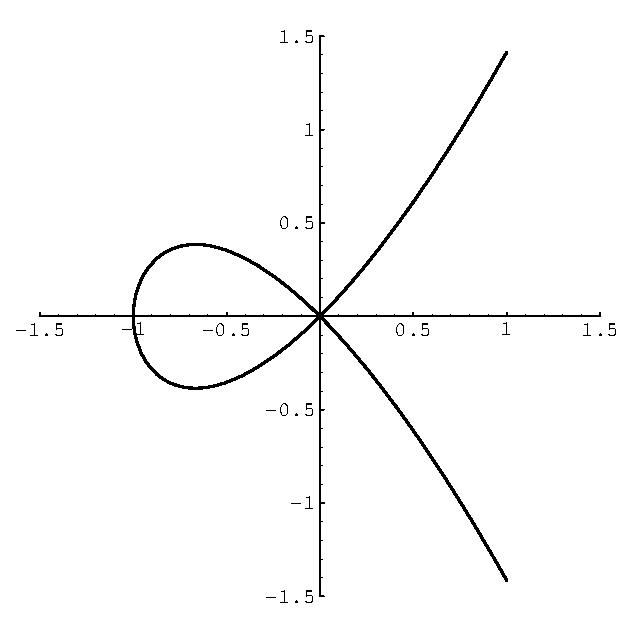
\includegraphics[width=2truein]{henselsg} &
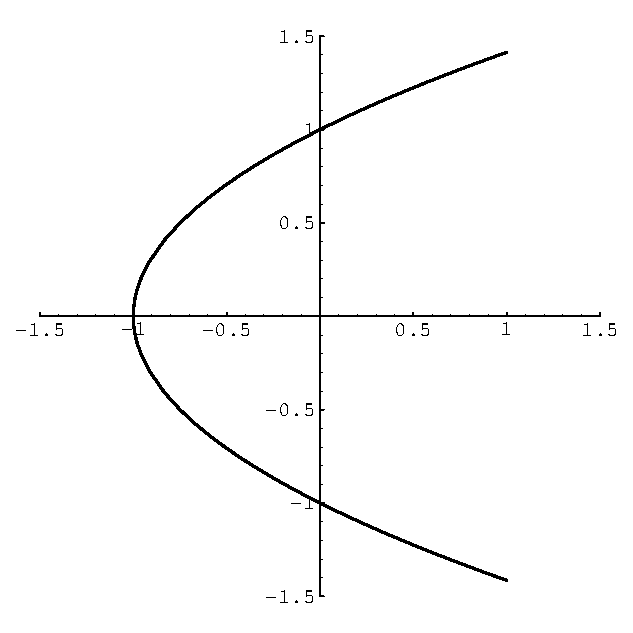
\includegraphics[width=2truein]{henselns} \\
(a) & (b)
\end{tabular}
\end{center}
\caption{The curves $Z^2 - t^3 -t^2$ and $Z^2 - t -1$
 \label{HenselSing:Fig}}
\end{figure}

As an example of what occurs when the derivative vanishes, consider
the polynomial
\[
F(Z) = Z^2 - t^2 - t^3,
\]
over the field $K = \Q(t)$.  If $F(Z)$ is square free and has two
distinct zeroes in $K_{(t)} = \Q((t))$:
\[
\begin{aligned}
\alpha & = t + \frac{t^2}{2} + \frac{t^3}{8} + \cdots, \\
\beta & =  - t - \frac{t^2}{2} - \frac{t^3}{8} - \cdots.
\end{aligned}
\]
However, modulo $\mathfrak{m} = (t)$ $F(Z)$ is not square free since the
constant terms of $\alpha$ and $\beta$ are the same.  

This situation is described geometrically in
\figref{HenselSing:Fig}(a).  In general, there are two points on the 
curve of $Z^2 - t^2 - t^3$ lying above any point on the horizontal,
$t$ axis.  At $t=0$ however, these two curve segments come together
at, what is called a \keyi{singular point} of the algebraic curve.

We can {\em desingularize} the curve at $t=0$, by focusing on the
second term in the power series expansion of $\alpha$ and $\beta$ not
the first.  That is, we replace $Z$ by $t Z'$.  This gives the new
equation:
\[
t^2 {Z'}^2 - t^2 -t^3 = 0.  
\]
So we can replace $F(Z)$ by $G(Z') = {Z'}^2 - 1 -t$.  This polynomial does
not have repeated roots modulo $\mathfrak{m}$ as is clear from
\figref{HenselSing:Fig}(b). 

More generally, assume that we have a polynomial $F(Z)$ over a ring
$R$ that is square free, but where $F(Z)$ is not square free over
$R/\mathfrak{p}$.  Further, assume that $\mathfrak{p} = (p)$ is a principal
ideal.  Since $F(Z)$ is not square free, it has more than one zero
lying over the point $\mathfrak{p}$ but which agree modulo $\mathfrak{p}$,
\eg,
\[
\begin{aligned}
\alpha & = a_0 + a_1 p + a_2 p^2 + a_3 p^3 + \cdots, \\
\beta  & = a_0 + b_1 p + b_2 p^2 + b_3 p^3 + \cdots.
\end{aligned}
\]
We can desingularize $F$ by using the new polynomial
\[
\frac{1}{p} F(p(Z - a_0))
\]
in place of $F(Z)$.  

The transformation described in the previous paragraph is called a
\keyi{blow up}.  It is known that blowup type transformations are
sufficient for desingularizing algebraic 
curves.\index{desingularization}  By repeatedly 
performing ``blow ups'' we can separate zeroes that agree modulo
$\mathfrak{p}^k$ for arbitrarily large, but finite $k$.  We can then
apply Newton's method to the desingularized equation to produce
approximations to the roots of arbitrary order.  

Note that if $F(Z)$ is not square free over $R$ then it is never
possible to separate the zeroes.

\section{Multidimensional Iteration}
\label{Multivariate:Newton:Sec}

Just as in the single variable case, the multivariate version of
Newton's iteration begins with \key{Taylor's formula}, this time in several
variables: Let $f(Z_1, \ldots, Z_n)$ be a polynomial in the variables
$Z_1, \ldots, Z_n$.  Its Taylor series expansion at $(x_1,\ldots,
x_n)$ is
\begin{equation}\label{Hensel:8}
\begin{aligned}
  \multispan{1}{$f(Z_1,\ldots, Z_n)$}\\
    \qquad = f(x_1,\ldots, x_n) &\null + 
    \sum_{i=1}^n {\partial f \over \partial Z_i}(x_1,\ldots,x_n) 
    (Z_i - x_i)\\
   & + {1 \over 2} \sum_{i=1}^n \sum_{j=1}^n
    {\partial^2 f \over \partial Z_i \, \partial Z_j}(x_1,\ldots,x_n) 
    (Z_i - x_i) (Z_j - x_j)\\
   & + \cdots\\
\end{aligned}
\end{equation}

The first summation in equation \eqnref{Hensel:8} is the inner product
of the row vector
\[
{\partial f \over \partial \vec{Z}} (\vec{x}) =
\left({\partial f \over \partial Z_1} (\vec{x}), 
{\partial f \over \partial Z_2} (\vec{x})
\ldots, {\partial f \over \partial Z_n} (\vec{x}) \right).
\]
and the column vector
\[
(\vec{Z} - \vec{x}) = \begin{pmatrix}Z_1 - x_1\\ \vdots\\ Z_n - x_n\end{pmatrix},
\]
where we have used $\vec{x}$ as an abbreviation for $(x_1, x_2, \ldots,
x_n)$ as in \sectref{Poly:Generalities:Sec}.  Using this notation, the
first two terms of \key{Taylor's formula} can be expressed as
\[
f(\vec{Z} ) = f(\vec{x}) + {\partial f \over \partial \vec{Z}}
(\vec{x}) \cdot (\vec{Z}  - \vec{x}) + \cdots.
\]

More generally, let $R$ be commutative ring, $\mathfrak{m}$ a maximal
ideal of $R$ and $\vec{f} = (f_1,\ldots,f_m)$ be a map from $R_\mathfrak{
m}^n$ to $R_\mathfrak{m}^m$.  It can be locally represented as a
multivariate power series expansion at $\vec{x}$
\[
\vec{f} (\vec{Z}) = \vec{f}(\vec{x}) 
  + \mathbf{J}(\vec{x})\cdot(\vec{Z} - \vec{x}) 
  + \cdots
\]
where $\mathbf{J}(\vec{x})$ is the \keyi{Jacobian} of the map $\vec{f}$:
\[
\mathbf{J}(\vec{x}) = 
\frac{\partial \vec{f}}{\partial \vec{Z}}
=
\begin{pmatrix}{\partial f_1\over \partial Z_1}& {\partial f_1\over \partial Z_2}&
 \cdots&{\partial f_1\over \partial Z_n}\\
{\partial f_2\over \partial Z_1}& {\partial f_2\over \partial Z_2}&
 \cdots&{\partial f_2\over \partial Z_n}\\
\vdots&\vdots&\ddots&\vdots\\
{\partial f_m\over \partial Z_1}& {\partial f_m\over \partial Z_2}&
 \cdots&{\partial f_m\over \partial Z_n}\end{pmatrix}.
\]
Again, letting $\vec{\alpha}$ be an element of the kernel of $\vec{f}$ and
expanding $\vec{f}$ at $\vec{\alpha} - \vec{\alpha}^{(k-1)}$, we have
\begin{equation}
0 = \vec{f}(\vec{\alpha}^{(k-1)}) + \mathbf{J}(\vec{\alpha}^{(k-1)}) 
\cdot (\vec{\alpha}  - \vec{\alpha}^{(k-1)}) +
O\left((\vec{\alpha} - \vec{\alpha}^{(k-1)})^{2}\right).
\label{MNewton:1:Eq}
\end{equation}

The term $O\left((\vec{\alpha} - \vec{\alpha}^{(k-1)})^{2}\right)$ is an
element of $\mathfrak{m}^{2}$.  If the rank of the Jacobian matrix is $n$
then the coordinates are well determined.  Choosing those rows of
\eqnref{MNewton:1:Eq} that are independent gives
\begin{equation}\label{MNewton:2:Eq}
\vec{\alpha}^{(2k-1)} - \vec{\alpha}^{(k-1)} 
  = -\mathbf{J}(\vec{\alpha}^{(k-1)})^{-1} 
  \cdot \vec{f}(\vec{\alpha}^{(k-1)}), \pmod{\mathfrak{m}^{2k}}
\end{equation}
which is quite similar to the quadratically convergent univariate iteration
\eqnref{Basic:UNewton:Eq}.  Equation \eqnref{MNewton:2:Eq} permits us to 
compute the element of 
$(R_\mathfrak{m})^n$ that lies over $\vec{\alpha_0}$.  However, this iteration
requires a matrix inversion at each step using a quadratically convergent 
iteration.  One way to eliminate the repeated matrix inversions is to use 
a linearly convergent version of \eqnref{MNewton:2:Eq}
\begin{equation}\label{MNewton:Lin:Eq}
\vec{\alpha}^{(k)} - \vec{\alpha}^{(k-1)}
   = -\mathbf{J}(\vec{\alpha}^{(0)})^{-1} 
  \cdot \vec{f}(\vec{\alpha}^{(k-1)}). \pmod{\mathfrak{m}^{k+1}}
\end{equation}

The linearly convergent iteration constructively shows that if the
Jacobian of a system of polynomial equations is invertible, a zero of
$\vec{f}(\vec{Z})$ modulo $\mathfrak{m}$ can always be lifted to a zero
modulo $\mathfrak{m}^k$ for any $k$.  That is,

\begin{proposition}\label{MNewton:Iter:Prop}
Assume $R$ is an integral domain with an ideal $\mathfrak{m}$.  Let
$\vec{f} = (f_1(Z_1, \ldots, Z_n), \ldots, f_n(Z_1, \ldots, Z_n))$ be
polynomials over $R$ and denote their Jacobian with respect to the
$Z_i$ by $\mathbf{J}$.  Let $(x_1, \ldots, x_n)$ be a zero of $\vec{f}$
modulo $\mathfrak{m}$ such that the determinant of $\mathbf{J}(x_1, \ldots,
x_n)$ has an inverse in $R/\mathfrak{m}$.  Then there exist unique
elements $\hat{x}_1, \ldots, \hat{x}_n$ of $R_\mathfrak{m}$, $\hat{x}_i =
x_i \mod\mathfrak{m}$, for which $\vec{f}(\hat{x}_1, \ldots, \hat{x}_n)
= 0$.
\end{proposition}

\begin{proof}
Let $\alpha_i^{(0)} = x_i$.  Since $\mathbf{J}(x_1, \ldots, x_n)$ is
invertible modulo $\mathfrak{m}$ we can repeatedly apply
\eqnref{MNewton:Lin:Eq} to compute $\vec{\alpha}^{(k)}$ for any
$k$.  The $\vec{\alpha}_i^{(k)}$ form a \key{coherent sequence} whose
limit is $\hat{x}_i$.

Thus there exists a point $(\hat{x}_1, \ldots, \hat{x}_n)$ that
satisfies the conditions of the proposition.  Assume that $(\hat{y}_1, 
\ldots, \hat{y}_n)$ also satisfies the proposition and that $k$ is the 
smallest value for which 
\begin{equation} \label{MNewton:NotEq:Eq}
\hat{x}_i \not= \hat{y}_i \pmod{\mathfrak{m}^{k+1}}
\end{equation}
for some $i$. Note that $k$ must be positive. We can denote by
$\vec{\alpha}^{(k-1)}$:
\[
(\hat{x}_1, \ldots, \hat{x}_n) = (\hat{y}_1, \ldots, \hat{y}_n) =
\vec{\alpha}^{(k-1)} \pmod{\mathfrak{m}^k}
\]
But then we have:
\[
\begin{aligned}
(\hat{x}_1, \ldots, \hat{x}_n) - \vec{\alpha}^{(k-1)}
   &= -\mathbf{J}(\vec{\alpha}^{(0)})^{-1} 
  \cdot \vec{f}(\vec{\alpha}^{(k-1)}), \\
(\hat{y}_1, \ldots, \hat{y}_n) - \vec{\alpha}^{(k-1)}
   &= -\mathbf{J}(\vec{\alpha}^{(0)})^{-1} 
  \cdot \vec{f}(\vec{\alpha}^{(k-1)}),
\end{aligned}
\pmod{\mathfrak{m}^{k+1}}
\]
which contradicts \eqnref{MNewton:NotEq:Eq}.
\end{proof}

\paragraph{Quadratic Iteration}

The need to repeatedly invert the Jacobian of the system can also be 
eliminated by applying Newton's method to the equation for the reciprocal 
of the Jacobian as described was done in
\sectref{Univariate:Newton:Sec}.\Marginpar{Rewrite this paragraph}
We apply \eqnref{MNewton:2:Eq} to the system linear of equations
\[
\mathbf{X} \cdot \mathbf{J}(\alpha) = {\bf 1}
\]
where both $\bf X$ and $\bf 1$ are $n\times n$ matrices, and the
components of $\bf X$ are to be determined.  Given
$\mathbf{\Upsilon}^{(k-1)}$ such that 
\[
\mathbf{\Upsilon}^{(k-1)} \cdot \mathbf{J}(\vec{\alpha}) = 
\mathbf{\Upsilon}^{(k-1)} \cdot \mathbf{J}(\vec{\alpha}^{(2k-1)}) = {\bf 1},
  \pmod{\mathfrak{m}^{k}}
\]
we want to find $\mathbf{\Upsilon}^{(2k-1)}$ where
\begin{equation} \label{Jacobian:1:Eq}
\mathbf{\Upsilon}^{(2k-1)} \cdot \mathbf{J}(\alpha^{(2k-1)}) = {\bf 1} \pmod{\mathfrak{m}^{2k}}
\end{equation}
We interpret the matrix equation \eqnref{Jacobian:1:Eq} as system of 
$n^{2}$ linear equations in $n^{2}$ unknowns, where the unknowns are the 
entries of $\mathbf{\Upsilon}^{(2k-1)}$. 

The Jacobian of \eqnref{Jacobian:1:Eq} is a block diagonal
$n^{2}\times n^{2}$ matrix, where each block contains
$\mathbf{J}(\alpha^{(2k-1)})^{T}$.  Since we only need to compute the
inverse of this matrix modulo $\mathfrak{m}^{k}$, we can write its
inverse as
\[
\begin{aligned}
\begin{pmatrix}
 \mathbf{J}(\alpha^{(2k-1)})^T & {\bf 0} & \cdots & {\bf 0}\\
 {\bf 0} & \mathbf{J}(\alpha^{(2k-1)})^T & \cdots & {\bf 0} \\
 \vdots  & & & \vdots \\
 {\bf 0} & {\bf 0} & \cdots & \mathbf{J}(\alpha^{(2k-1)})^T \end{pmatrix}^{-1} \qquad\\
 = 
\begin{pmatrix}
 \mathbf{\Upsilon}^{(k-1) \, T} & {\bf 0} & \cdots & {\bf 0}\\
 {\bf 0} & \mathbf{\Upsilon}^{(k-1) \, T} & \cdots & {\bf 0} \\
 \vdots  & & & \vdots \\
 {\bf 0} & {\bf 0} & \cdots & \mathbf{\Upsilon}^{(k-1) \, T} \end{pmatrix}
\end{aligned}
\pmod{\mathfrak{m}^{k}}
\]
According to \eqnref{MNewton:2:Eq}, $\vec{\mathbf{J}}^{(2k-1)} - \vec{\mathbf{J}}^{(k)}$
is equal to the product of this matrix multiplied on the right by the
vector of entries of 
\[
\mathbf{\Upsilon}^{(k-1)} \cdot \mathbf{J}(\alpha^{(2k-1)}) - {\bf 1} \pmod{\mathfrak{m}^{2k}}.
\]
Due to the repetitive structure of the Jacobian, we can write this as 
\begin{equation}
\mathbf{\Upsilon}^{(2k-1)} - \mathbf{\Upsilon}^{(k-1)} =
({\bf 1} - \mathbf{\Upsilon}^{(k-1)} \cdot \mathbf{J}(\vec{\alpha}^{(2k-1)})) \cdot 
\mathbf{\Upsilon}^{(k-1)} \pmod{\mathfrak{m}^{2k}}
\label{MNewton:3:Eq}
\end{equation}

Putting this together with \eqnref{MNewton:2:Eq} we have
\begin{equation}
\label{Quasi:MNewton:Eq}
 \begin{aligned}
   \vec{\alpha}^{(2k-1)} - \vec{\alpha}^{(k-1)} & 
      = -\mathbf{\Upsilon}^{(k-1)}\cdot \vec{f}(\vec{\alpha}^{(k-1)}) \\
   \mathbf{\Upsilon}^{(2k-1)} - \mathbf{\Upsilon}^{(k-1)} &=
     ({\bf 1} - \mathbf{\Upsilon}^{(k-1)} \cdot \mathbf{J}(\vec{\alpha}^{(2k-1)})) 
          \cdot \mathbf{\Upsilon}^{(k-1)}
 \end{aligned}
 \pmod{\mathfrak{m}^{2k}}
\end{equation}
which is the basic quadratically convergent multivariate iteration.

To illustrate the steps leading from \eqnref{Jacobian:1:Eq} to
\eqnref{MNewton:3:Eq}, we consider the $2 \times 2$ case explicitly:
\[
\begin{aligned}
\mathbf{X}^{(2k-1)} \cdot \mathbf{M}^{(2k-1)} 
& = 
\begin{pmatrix}x_{11}^{(2k-1)} & x_{12}^{(2k-1)} \\\noalign{\vskip3pt}
x_{21}^{(2k-1)} & x_{22}^{(2k-1)} \end{pmatrix} 
\cdot
\begin{pmatrix}m_{11}^{(2k-1)} & m_{12}^{(2k-1)} \\\noalign{\vskip3pt}
m_{21}^{(2k-1)} & m_{22}^{(2k-1)} \end{pmatrix} \\
& = \begin{pmatrix}1& 0 \\ 0 & 1 \end{pmatrix},
\end{aligned}
\pmod{\mathfrak{m}^{2k}}
\]
where $\mathbf{M}^{(2k-1)}$ is the image modulo $\mathfrak{m}^{2k}$ of a
known matrix $\mathbf{M}$ and $\mathbf{X}^{(2k-1)}$ is a matrix whose elements
are to be determined.  The correspondence to our case is
$\mathbf{X}^{(2k-1)} = \mathbf{\Upsilon}^{(2k-1)}$ and $\mathbf{M}^{(2k-1)} =
\mathbf{J}(\vec{\alpha}^{(2k-1)})$. In terms of their components, these
equations are 
\[
\begin{aligned}
 f_1(x_{11}, x_{12}, x_{21}, x_{22}) & 
   = m_{11} x_{11} + m_{21} x_{12} - 1, \\
 f_2(x_{11}, x_{12}, x_{21}, x_{22}) & 
   = m_{12} x_{11} + m_{22} x_{12}, \\ 
 f_3(x_{11}, x_{12}, x_{21}, x_{22}) & 
   = m_{11} x_{21} + m_{21} x_{22}, \\ 
 f_4(x_{11}, x_{12}, x_{21}, x_{22}) & 
   = m_{12} x_{21} + m_{22} x_{22} - 1,
\end{aligned}
\]
which gives a Jacobian of 
\[
\begin{pmatrix}
   m_{11} & m_{21} & 0 & 0 \\
   m_{12} & m_{22} & 0 & 0 \\
   0 & 0 & m_{11} & m_{21} \\
   0 & 0 & m_{12} & m_{22} \end{pmatrix}.
\]
Using \eqnref{MNewton:2:Eq}, the quadratic iteration for the solution
of this system of equations is
\[
\begin{aligned}
\null & \begin{pmatrix}
  x_{11}^{(2k-1)} - x_{11}^{(k-1)} \\
  x_{12}^{(2k-1)} - x_{12}^{(k-1)} \\
  x_{21}^{(2k-1)} - x_{21}^{(k-1)} \\
  x_{22}^{(2k-1)} - x_{22}^{(k-1)} \end{pmatrix} \\
\null & \qquad =
- \begin{pmatrix}
   j_{11}^{(k-1)} & j_{21}^{(k-1)} & 0 & 0 \\
   j_{12}^{(k-1)} & j_{22}^{(k-1)} & 0 & 0 \\
   0 & 0 & j_{11}^{(k-1)} & j_{21}^{(k-1)} \\
   0 & 0 & j_{12}^{(k-1)} & j_{22}^{(k-1)} \end{pmatrix}
\cdot
\begin{pmatrix}
  f_1(\vec{x}^{(k-1)}) \\ 
  f_2(\vec{x}^{(k-1)}) \\
  f_3(\vec{x}^{(k-1)}) \\ 
  f_4(\vec{x}^{(k-1)}) \end{pmatrix} \\
\null & \qquad = - \begin{pmatrix}
    j_{11}^{(k-1)}f_1(\vec{x}^{(k-1)}) + j_{21}^{(k-1)}f_2(\vec{x}^{(k-1)})\\
    j_{12}^{(k-1)}f_1(\vec{x}^{(k-1)}) + j_{22}^{(k-1)}f_2(\vec{x}^{(k-1)})\\
    j_{11}^{(k-1)}f_3(\vec{x}^{(k-1)}) + j_{21}^{(k-1)}f_4(\vec{x}^{(k-1)})\\
    j_{12}^{(k-1)}f_3(\vec{x}^{(k-1)}) + j_{22}^{(k-1)}f_4(\vec{x}^{(k-1)})
    \end{pmatrix}
\\
\end{aligned}
\pmod{\mathfrak{m}^{2k}}
\]
This can be rewritten as a product of $2 \times 2$ matrices as 
\[
\begin{aligned}
\null & \begin{pmatrix}
  x_{11}^{(2k-1)} - x_{11}^{(k-1)} &
  x_{12}^{(2k-1)} - x_{12}^{(k-1)} \\
  x_{21}^{(2k-1)} - x_{21}^{(k-1)} &
  x_{22}^{(2k-1)} - x_{22}^{(k-1)} \end{pmatrix} \\
\null & \qquad =
\begin{pmatrix}
  f_1(\vec{x}^{(k-1)}) & f_2(\vec{x}^{(k-1)}) \\
  f_3(\vec{x}^{(k-1)}) & f_4(\vec{x}^{(k-1)}) \end{pmatrix}
\cdot
\begin{pmatrix}
   j_{11}^{(k-1)} & j_{12}^{(k-1)} \\
   j_{21}^{(k-1)} & j_{22}^{(k-1)} \end{pmatrix}
\end{aligned}
\]


The initial solution of the system of equations, $\vec{\alpha}_{0}$ is
called the starting point of the iteration.  If
$\mathbf{J}(\vec{\alpha}_0)$ is invertible then $\vec{\alpha}_0$ is said
to be a \keyi{good starting point}.  If the Jacobian matrix is not
invertible, either because the $\vec{\alpha}_0$ was a bad starting
point or because the Jacobian itself was not square, then the system
of linear equations that need to be solved at each step will not have a
unique solution.  There are cases where this can be useful, for
instance as a sieve for possible solutions to diophantine 
equations\index{diophantine equation}
over the integers.

\section{Hensel's Lemma}
\label{Hensel:Lemma:Sec}
\index{Hensel's lemma|(}

One of the the most useful theorems in commutative algebra is {\em
Hensel's lemma}.  Essentially, it says that if a monic polynomial with
coefficients in a ring $R$ factors modulo an ideal $\mathfrak{m}$, then
it factors as a polynomial over $R_\mathfrak{m}$.  More precisely,

\begin{proposition}[Hensel's Lemma] \label{Hensel:Lemma:Prop}
Let $F(Z)$ be a monic polynomial over an integral domain $R$,
$\mathfrak{m}$ an ideal of $R$.  If there exist polynomials $G(Z)$ and
$H(Z)$ over $R/\mathfrak{m}$ such that 
\[
F(Z) = G(Z) H(Z) \pmod\mathfrak{m}
\]
and $G(Z)$ and $H(Z)$ are relatively prime as polynomials over
$R/\mathfrak{m}$, then there exist polynomials $\hat{G}(Z)$ and
$\hat{H}(Z)$ over $R_\mathfrak{m}$ such that
\[
\begin{aligned}
G(Z) & = \hat{G}(Z) \\ H(Z) & = \hat{H}(Z)
\end{aligned}
\pmod\mathfrak{m}
\]
and $F(Z) = \hat{G}(Z) \hat{H}(Z)$ over $R_\mathfrak{m}$.
\end{proposition}

Although, this proposition is phrased in terms of polynomials in $R[Z]$, 
the variable $Z$ is only used as a place holder that allows us to 
succinctly describe a system of non-linear equations.  This is clarified 
in the following proof. 

\begin{proof}
Let the degree of $F$ in $Z$ be $d$ and that of $G(Z)$ and $H(Z)$ be
$r$ and $s$ respectively, $r+s = d$.  We denote the coefficients of
$F$ by $f_i$,
\[
F(Z) = Z^d + f_1 Z^{d-1} + \cdots + f_d,
\]
where $f_i \in R$.  And the coefficients of $G$ and $H$ by $g^{(0)}_i$
and $h^{(0)}_i$:
\[
\begin{aligned}
G(Z) &= Z^r + g^{(0)}_1 Z^{r-1} + \cdots + g^{(0)}_r, \\
H(Z) &= Z^s + h^{(0)}_1 Z^{s-1} + \cdots + h^{(0)}_s,
\end{aligned}
\]
where $g^{(0)}_i$ and $h^{(0)}_i$ are elements of $R/\mathfrak{m}$.

If $G$ and $H$ can be lifted to polynomials over
$R_\mathfrak{m}$, then we can write
\[
\begin{aligned}
\hat{G}(Z) & = Z^r + g_1 Z^{r-1} + \cdots + g_r, \\
\hat{H}(Z) & = Z^s + h_1 Z^{s-1} + \cdots + h_s, 
\end{aligned}
\]
where $g_i$ and $h_i$ are unknown elements of $R_\mathfrak{m}$.
Expanding $\hat{G}(Z) \hat{H}(Z) = F(Z)$ and equating coefficients of
$Z$ we have
\begin{equation}\label{Hensel:Eq}
\begin{aligned}
  g_1 + h_1&= f_1,\\
  g_2 + g_1h_1 + h_2&= f_2,\\
  \vdots&\\
  g_r h_{s-1} + g_{r-1} h_s&= f_{n-1},\\
  g_r h_s&= f_n.
\end{aligned}
\end{equation}
This is a system of $d$ equations if $r+s$ unknowns and is called the
\keyi{coefficient equations} of the factorization $F = \hat{G}\cdot
\hat{H}$.  Any factorization of $F(Z)$ into factors of degree $r$ and
$s$ leads to a solution of \eqnref{Hensel:Eq}.  Conversely, any
solution of \eqnref{Hensel:Eq} leads to a factorization of $F(Z)$.
Thus solving \eqnref{Hensel:Eq} and factoring $F(Z)$ are equivalent. 

The coefficients of $G(Z)$ and $H(Z)$ are a solution of
\eqnref{Hensel:Eq} modulo $\mathfrak{m}$.  By \propref{MNewton:Iter:Prop} this
solution can be uniquely lifted to a solution in $R_\mathfrak{m}$ if the
Jacobian of \eqnref{Hensel:Eq} is non-singular.

The Jacobian of \eqnref{Hensel:Eq} can be computed directly:
\[
\left(
\begin{array}{cccccccc}
  1 &   0 & \ldots &   0 &   1 &   0 & \ldots & 0 \\
h_1 &   1 &        &   0 & g_1 &   1 &        & 0 \\
h_2 & h_1 & \ldots &   0 & g_2 & g_1 & \ldots & 0 \\
\vdots&   &        &     & \vdots&   &        &\vdots\\
0   &   0 & \ldots & h_s & 0   &   0 & \ldots &g_r
\end{array}
\right),
\]
the \key{Sylvester matrix} for the \key{resultant} of $G(Z)$ and
$H(Z)$, as was pointed out in \sectref{Poly:Resultant:Sec}.  It is
known to be zero if and only if $g$ and $h$ have a nontrivial common
factor.  Since $G(Z)$ and $H(Z)$ are assumed to be relatively prime,
the Jacobian is always non-singular.
\end{proof}

\paragraph{Example}

Consider the polynomial 
\[
F(Z) = Z^5 +Z^4 + 2Z^2 + 2Z + 3.
\]
Modulo $5$ it can be factored
\begin{equation}\label{Hensel:Ex5:Eq}
F(Z) = (Z^3 + 4Z + 3) (Z^2 + Z + 1) \pmod{5}
\end{equation}
Suspecting that $F(Z)$ factors into a quadratic and a cubic factor
over the rational integers we use \longpropref{Factor:CBound:Prop} to
bound the size of the coefficients of its factors.  If $G$ and $H$ are
the cubic and quadratic factors of $F$ over the integers, then
\[
(d+1)^{1/2} 2^d |F| = \sqrt{6}\, 2^5\times 3 \approx 8465 \ge \max \{
|G|, |H|\}.
\]
So we should lift the factorization of $F(Z)$ to one modulo $5^7 > 2
\times 9000$.

The \keyi{coefficient equations} corresponding to the factorization of
$F(Z)$ into a cubic and quadratic factor are
\begin{equation} \label{MNewton:Sing:Eq}
\begin{aligned}
a_1 + b_1 & = 1, \\
a_2 + a_1 b_1 + b_2 & = 0, \\
a_3 + a_2 b_1 + a_1 b_2 & = 2, \\
a_3 b_1 + a_2 b_2 & = 2, \\
a_3 b_2 & = 3.
\end{aligned}
\end{equation}
The Jacobian of this system of equations is 
\[
\left(
\begin{array}{ccccc}
1 & 0 & 0 & 1 & 0 \\
b_1 & 1 & 0 & a_1 & 1 \\
b_2 & b_1 & 1 & a_2 & a_1 \\
0   & b_2 & b_1 & a_3 & a_2 \\
0   & 0   & b_2 & 0   & a_3
\end{array}
\right).
\]
We can verify that this matrix is non-singular when the $a_i$ and
$b_i$ are replaced by their corresponding values from
\eqnref{Hensel:Ex5:Eq}.  By applying the multivariate version of Newton's
iteration \eqnref{MNewton:Lin:Eq} we get 
\[
\begin{aligned}
a_1 & = 0 + 0\cdot 5 + 0 \cdot 5^2 + 0 \cdot 5^3 + \cdots, \\
a_2 & = 6 + 6\cdot 5 + 6 \cdot 5^2 + 6 \cdot 5^3 + \cdots, \\
a_3 & = 3 + 0\cdot 5 + 0 \cdot 5^2 + 0 \cdot 5^3 + \cdots, \\
b_1 & = 1 + 0\cdot 5 + 0 \cdot 5^2 + 0 \cdot 5^3 + \cdots, \\
b_2 & = 1 + 0\cdot 5 + 0 \cdot 5^2 + 0 \cdot 5^3 + \cdots. \\
\end{aligned}
\]

Modulo $7$ however we get the factorization
\[
f(Z) = (Z^3 + 6 Z + 3) (Z^2 +  Z + 1).
\]
These factors are not irreducible and share a common factor of
$X+3$.  The Jacobian in this case is 
\[
\left(
\begin{array}{ccccc}
1 & 0 & 0 & 1 & 0 \\
1 & 1 & 0 & 0 & 1 \\
1 & 1 & 1 & 6 & 0 \\
0 & 1 & 1 & 3 & 6 \\
0 & 0 & 1 & 0 & 3
\end{array}
\right),
\]
whose integer determinant is $4 \times 7$.

\label{PolyZ7:SQFR:Ex}
Although $F(Z)$ is not square free over $\Z/(7)$ it does have three
distinct zeroes in $\Z_7$:
\[
\begin{aligned}
\alpha_1 & = 4 + 2\cdot 7 + 0\cdot 7^2 + 3\cdot 7^3 + 6\cdot 7^4 +
4\cdot 7^5 + 0\cdot 7^6 + 4\cdot 7^7 + \cdots \\
\alpha_2 & = 4 + 1\cdot7 + 3\cdot7^2 + 6\cdot7^3 + 0\cdot7^4 + 2\cdot7^5
+ 5\cdot7^6 + 1\cdot7^7 + \cdots \\
\alpha_3 & = 2 + 4\cdot7 + 6\cdot7^2 + 3\cdot7^3 + 0\cdot7^4 +
2\cdot7^5 + 6\cdot7^6 + 2\cdot7^7 + \cdots
\end{aligned}
\]
This explains the indeterminacy of the factorization.  The quadratic
factor could be either
\[
(Z - \alpha_1) \cdot (Z - \alpha_3) \quad\mbox{or}\quad
(Z - \alpha_2) \cdot (Z - \alpha_3).
\]
Both factorizations have the same image modulo $7$.  Since $7^2$ does
not divide the determinant of the Jacobian, these two factorizations
can be differentiated by their images modulo $7^2$.

The system of equations \eqnref{MNewton:Sing:Eq} describes an
algebraic surface embedded in a five dimensional space.  The fact that
the Jacobian is divisible by $7$ means that the surface has a singular
point at $(7)$.  It is possible to desingularize surface by blow ups
as described in the unvariate case,\index{desingularization} \index{blow 
up} but the discussion would take us too far a field.

\index{Hensel's lemma|)}

\section{Generalizations of Hensel's Lemma}
\label{General:Hensel:Sec}

While Hensel's lemma is usually expressed in terms of factoring a
polynomial into two relatively prime factors, the technique given in
the previous section can be applied more generally. 

Consider what happens if $F(Z)$ has three factors modulo
$\mathfrak{m}$, \ie, $F(Z) = A(Z) \cdot B(Z) \cdot C(Z)$ modulo
$\mathfrak{m}$ and $A(Z)$, $B(Z)$, and $C(Z)$ have degrees $r_1$,
$r_2$ and $r_3$ respectively, $r = r_1 + r_2 + r_3$.  We then know
that
\[
\begin{aligned}
  Z^r + \cdots + f_r&=
    (Z^{r_1} + \cdots + a_{r_{1}}) (Z^{r_2} + \cdots + b_{r_{2}})
    (Z^{r_3} + \cdots + c_{r_{3}}),\\
   &= Z^{r_1 + r_2 + r_3} + (a_{1} + b_{1} + c_{1}) Z^{r_1 + r_2 + r_3 -1} 
    + \cdots + a_{r_{1}} b_{r_{2}} c_{r_{3}}.
\end{aligned}
\]
If we equate the coefficients $Z^i$ on the right hand side of the
equation with those on the left hand side, we get a system of $r = r_1 + 
r_2 + r_3$ algebraic equations in $r$ unknowns.  The Jacobian of this 
system is a $r\times r$ matrix, $\mathbf{J}_1$ whose first $r_1$ columns 
look like 
\[
\overbrace{
\begin{array}{cccc}
1 & 0 & \cdots  & 0 \\
b_1 + c_1 & 1 & \cdots & 0\\
b_2 + b_1 c_1 + c_2 & b_1 + c_1 &  \cdots & 0 \\
\vdots & & & \vdots \\
0 & 0 & \cdots & b_{r_2} c_{r_3} \\
\end{array}}^{r_1}
\]
The next $r_2$ and $r_3$ columns are organized similarly.  By
\propref{MNewton:Iter:Prop}, when $\mathbf{J}_1$ is invertible over
$R/\mathfrak{m}$ the factorization $F = A \cdot B \cdot C$ can be lifted
{\em uniquely} to a factorization of $F$ in $R_\mathfrak{m}$.  When there
are just two factors, non-singularity of the Jacobian corresponds to
the factors being relatively prime.  What criteria corresponds to the
invertibility of $\mathbf{J}_1$?

If $A(Z)$ and $B(Z)$ are not relatively prime modulo $\mathfrak{m}$, then
the lift is certainly not unique, and similarly for the other pairings.
Thus, we expect that
\[
R = (\res_Z (A(Z), B(Z))) \cdot (\res_Z (A(Z), C(Z))) 
  \cdot (\res_Z (B(Z), C(Z)))
\]
divides the determinant of $\mathbf{J}_1$.  The term with maximum total 
degree in $R$ has total degree 
\[
(r_1 + r_2 - 1) + (r_1 + r_3 - 1) + (r_2 + r_3 - 1) = 2r -3.
\]
Examining the degrees of the rows of $\mathbf{J}_1$ we see that the monomial
of maximum total degree in 
the determinant of $\mathbf{J}_1$ has total degree
\[
0 + 1 + \overbrace{2 + 2 + \cdots + 2}^{r-2} = 2r -3.
\]
Thus,
\[
\det \mathbf{J}_1 = (\res_Z (A(Z), B(Z))) \cdot (\res_Z (A(Z), C(Z))) 
  \cdot (\res_Z (B(Z), C(Z))).
\]
Similar reasoning extends this result to an arbitrary number of
pairwise relatively prime factors.  

\smallskip
More generally, assume we have a monic polynomial $F(Z)$ over a ring
$R$ that has a factorization
\begin{equation} \label{Hensel:NSQ:Eq}
F(Z) = P_1^{e_1}(Z) \cdot P_2^{e_2}(Z) \cdots P_n^{e_n}(Z)
\pmod{\mathfrak{m}}
\end{equation}
The previous paragraphs discussed the case when the $e_i$ are equal to
$1$.  The coefficient equations of this factorization can be formed in
the same way as in the previous discussion.  Now, however, the number
equations exceeds the number unknowns.  Since there is a one to one
correspondence between factorizations $F(Z)$ of the form
\eqnref{Hensel:NSQ:Eq} and zeroes of the system of coefficient
equations, the coefficient equations must be consistent.

An interesting illustration of this approach is to lift the
factorization 
\[
\begin{aligned}
F(Z) & = Z^5 + Z^4 + 2Z^2 + 2Z + 3, \\
  & = (Z+3)^2 (Z+5) (Z^2 + 4Z+1),
\end{aligned}
\pmod{7}
\]
to a factorization over $\Z_7$.  On page \pageref{PolyZ7:SQFR:Ex} we showed that as
a polynomial over $\Z_7$ $F(Z)$ was square free.  Thus, this
factorization cannot be lifted to a factorization over $\Z_7$. Here we
show how the lifting process breaks down. possible since earlier $F(Z)$ was shown to be square free over $\Z_7$.

Assuming that
\begin{equation} \label{Hensel:NSQEx:Eq}
F(Z) =  (Z + a)^2  (Z+b) (Z^2+c_1Z+c_2)
\end{equation}
The coefficient equations are 
\[
\begin{aligned}
2a + b + c_1 & = 1, \\
a^2 + 2ab + 2 ac_1 + b c_1 + c_2 & = 0, \\
a^2 b + a^2 c_1 + 2 a b c_1 + 2 a c_2 + b c_2 & = 2, \\
a^2 b c_1 + a^2 c_2 + 2 a b c_2 & = 2, \\
a^2 b c_2 & = 3.
\end{aligned}
\]
The Jacobian of the first four equations, at $(a,b,c_1,c_2) =
(3,5,4,1)$ has integer determinant $48$.  Its inverse modulo $7$ is
\[
\left(
\begin{array}{cccc}
3 & 1 & 6 & 6 \\
4 & 0 & 3 & 4 \\
5 & 5 & 6 & 5 \\
1 & 6 & 5 & 6 
\end{array}
\right).
\]
Thus, we can uniquely lift the zero to a zero of the first four
equations in $\Z_7$:
\[
\begin{aligned}
a   & = 3 +         7 + 0 \cdot 7^2 + 6 \cdot 7^3 + 5 \cdot 7^4 + \cdots, \\
b   & = 5 + 2 \cdot 7 + 2 \cdot 7^2 + 1 \cdot 7^3 + 4 \cdot 7^4 + \cdots, \\
c_1 & = 3 + 1 \cdot 7 + 4 \cdot 7^2 + 0 \cdot 7^3 + 5 \cdot 7^4 + \cdots, \\
c_2 & = 1 + 3 \cdot 7 + 1 \cdot 7^2 + 1 \cdot 7^3 + 0 \cdot 7^4 +
\cdots.
\end{aligned}
\]
Unfortunately, this solution is not a zero of the final equation.
There the coefficient equations do not have a solution in $\Z_7$, just
as the polynomial $F(Z)$ does not have a factorization of the form
\eqnref{Hensel:NSQEx:Eq}.

\medskip
The {\sc gcd} problem can be handled in a similar manner.  Assume
we want to compute $H(Z)$, which is the {\sc gcd} of $F(Z)$ and $G(Z)$,
where $\deg F = r$, $\deg G = s$ and $\deg H = n$.  Letting $F(Z) =
A(Z) H(Z)$ and $G(Z) = B(Z) H(Z)$ we get the following system of
equations:
\[
\begin{aligned}
  a_1 + h_1 &= f_1\\
  a_2 + a_1 h_1 + h_2 &= f_2 \\
  \vdots\\
  a_{r - n} h_n & = f_r
\end{aligned} \qquad
\begin{aligned}
  b_1 + h_1 &= g_1\\
  b_2 + a_1 h_1 + h_2 &= g_2 \\
  \vdots\\
  b_{s - n} h_n & = g_r
\end{aligned}
\]
We now have $r+s$ equations, but only have $n + r -n + s - n = r + s
-n$ unknowns.  Thus, some of these equations are redundant if $F$
and $G$ actually have a unique {\sc gcd} of degree $n$.  Notice that
applying the Hensel approach to the {\sc gcd} problem gives a method
that lifts, not only $H$, but also the cofactors of $F$ and 
$G$.\index{cofactor} 

\section{Zassenhaus' Formulation of Hensel's Lemma}
\label{Zassenhaus:Formulation:Sec}

{\Zassenhaus}' version of \key{Hensel's lemma} differs from the one
discussed in the preceding sections in that the number of equations
produced is smaller than the number of variables.  For instance, in
the factoring problem, the Zassenhaus approach determines $G$ and $H$
by solving the equation
\begin{equation}
 \label{Zassen:Factor:Eq}
F(X) - G(X) \cdot H(X) = 0
\end{equation}
It is only when the solution of this equation is restricted to the ring
$\Z_{p}[X]$ that \eqnref{Zassen:Factor:Eq} has a unique solution.  By using
a $p$-adic technique the non-linear diophantine equation
\eqnref{Zassen:Factor:Eq} can be reduced to a series of easy to solve,
linear equations.  Then by piecing together the solutions of these linear
equations, $G$ and $H$ can be determined.  Here we outline the main 
points and demonstrate the connection with our formalism.

Let $F(X)$ be a univariate polynomial over the integers, and assume
that it has two irreducible factors, $G$ and $H$.  We are given a
factorization $F(X) = G_0 H_0$ modulo $p$ and we want to lift $G_0$
and $H_0$ to $G$ and $H$.  Writing $G$ and $H$ $p$-adically gives
\[
\begin{aligned}
  F(X) &= (G_0 + G_1 p + \cdots) (H_0 + H_1 p + \cdots), \\
   &= G_0 H_0 + (H_1 G_0 + G_1 H_0) p + \cdots.
\end{aligned}
\]
Modulo $p^2$ we have
\[
F(X) - G_0 H_0 = (H_1 G_0 + G_1 H_0) p \pmod{p^2}
\]
Since $F(X) - G_0 H_0$ is a multiple of $p$, dividing by $p$ gives 
\begin{equation}
H_1 G_0 + G_1 H_0 = \left( F(X) - G_0 H_0 \right) / p \qquad\pmod{p}
\label{Linear:Dio:Eq}
\end{equation}
This is a polynomial valued linear diophantine equation\index{diophantine 
equation!linear} in $G_1$ and $H_1$.  Its solution can be obtained by 
first solving $A_i G_0 + B_i H_0 = X^i \pmod{p}$ for various $i$ by the 
Euclidean algorithm.  Since the left hand side of \eqnref{Linear:Dio:Eq} 
is a polynomial in $X$, $G_1$ and $H_1$ can be determined by adding 
combinations of the appropriate $B_i$ and $A_i$ respectively.

Having computed $G_1$ and $H_1$, the other terms may be computed
similarly.  For a linear iteration, the process continues as follows:
\[
F(X) = (G_0 + G_1 p + G_2 p^2 + \cdots) 
(H_0 + H_1 p + H_2 p^2 + \cdots)
\]
Considering this equation modulo $p^3$
\[
(H_2 G_0 + G_2 H_0) = \left( F(Z) - 
  (G_0 + G_1 p)(H_0 + H_1 p) \right) / p^2 \qquad \pmod{p}
\]
The right hand side of this equation is again a polynomial and the
left hand side is essentially the same as \eqnref{Linear:Dio:Eq}.  So
using the $A_i$ and $B_i$ obtained in the previous step we can compute
$G_2$ and $H_2$.

\paragraph{Relation to Solving Equations}

The {\Zassenhaus} version of \key{Hensel's lemma} produces the same 
answer as the approach based on Newton's method discussed earlier---the 
correct factorization through each of the lifting stages.  The
following paragraphs demonstrate that this is not a fortuitous
accident but is due to the fact that both formulations are performing
the same computation in a slightly different manner.

The key to using {\Zassenhaus}'s formulation of \key{Hensel's lemma} to 
lift a factorization $F = G_0 H_0 \mod{\mathfrak{m}}$ to the $\mathfrak{
m}$-adic completion is solving the diophantine equations
\begin{equation} \label{Hensel:ZassDio:Eq}
A_i G_0 + B_i H_0 = Z^i \qquad\pmod{\mathfrak{m}}
\end{equation}
Once we have obtained the $A_i$ and $B_i$, it is merely a matter of
computing the error introduced when a factorization modulo $\mathfrak{m}^k$ 
is lifted to one modulo $\mathfrak{m}^{k+1}$.
This error is then used to produce the appropriate linear combination of the
$A_i$ and $B_i$ that is $G_{k+1}$ and  $H_{k+1}$.

Our formulation is quite similar.  We begin by inverting the Jacobian
matrix.  Through the Newton-Raphson formula we combine the error terms
to compute $G_{k+1}$ and $H_{k+1}$.  Structurally, these two algorithms 
are quite similar.  We shall see that the solutions of 
\eqnref{Hensel:ZassDio:Eq} form the inverse of the Jacobian matrix.

To see this let,
\[
\begin{aligned}
  G_0 &= Z^r + g_1 Z^{r-1} + g_2 Z^{r-2} + \cdots + g_r\\
  H_0 &=Z^s + h_1 Z^{s-1} + h_2 Z^{s-2} + \cdots + h_s
\end{aligned}
\]
so the Jacobian matrix is
\[
J = 
\begin{pmatrix}
1&0&0& \cdots&0&1&0&0&\cdots&0\\
h_1&1&0& \cdots&0&g_1&1&0&\cdots&0\\
h_2&h_1&1& \cdots&0&g_2&g_1&1&\cdots&0\\
\vdots&\null&\vdots&\null&\null&\vdots&\null&\vdots&\null&\vdots\\
0&\cdots&0&h_s&h_{s-1}&0&\cdots&0&g_r&g_{r-1}\\
0&\cdots&0&0&h_s&0&\cdots&0&0&g_r
\end{pmatrix}
\]
Consider what happens when this matrix is multiplied by a column vector
\[
J\cdot
\begin{pmatrix}
b_0\\ \vdots \\ b_{s-1}\\ a_0\\ \vdots\\ a_{r-1}
\end{pmatrix}
=
\begin{pmatrix}
a_0 +b_0\\
a_0 g_1 + a_1 + b_1 + b_0 h_1\\
\vdots\\
a_{r-1} g_{r-1} + a_{r-2} g_r + b_{s-2} h_{s} + b_{s-1} h_{s-1}\\
a_{r-1} g_{r} + b_{s-1} h_{s}
\end{pmatrix}
\]
The $(r+ s - 1) - i$ row of this column vector is clearly the coefficient
of $Z^i$ in $A G_0 + B H_0$ where
\[
\begin{aligned}
  A &= a_0 Z^{s-1} + a_1 Z^{s-2} + \cdots + a_{s-1},\\
  B &= b_0 Z^{r-1} + b_1 Z^{r-2} + \cdots + b_{r-1}.
\end{aligned}
\]
Thus the computation of the inverse of the Jacobian of the system of
equations is a clever way of obtaining all the solutions of
\eqnref{Hensel:ZassDio:Eq}.  Or, solving
\eqnref{Hensel:ZassDio:Eq} is a clever way of inverting a very special
type of Jacobian matrix.

\section*{Notes}

\small

\notesectref{Univariate:Newton:Sec}  Equation
\eqnref{Basic:UNewton:Eq} is a discrete version of the Newton-Raphson
iteration used in numerical analysis.  Unlike the numerical situation,
notice that convergence in the discrete case is is not an issue.  The
linearly convergent iteration \eqnref{Modified:UNewton:Eq} is called a
\keyi{modified Newton's method} in numerical analysis.

An alternative approach to Hensel's lemma liftings, but based on the
use of idempotents is given in the work of {\Gianni}, {\MillerV} and
{\Trager} \cite{Gianni1989-dd}.

\notesectref{Multivariate:Newton:Sec} In a certain sense this is a
discrete version of a \keyi{quasi-Newton iteration}, since it updates
the Jacobian at each step rather than recomputing it.  However, most
of the numerical quasi-Newton formulas do not update the entire matrix
as is done in \eqnref{MNewton:2:Eq}.

\notesectref{Hensel:Lemma:Sec} A result equivalent to Hensel's lemma
was first proven in \cite{Hensel04,Hensel05a}.  It was given in the
form of \propref{Hensel:Lemma:Prop} in \cite{Hensel1918-mx}.

\notesectref{Zassenhaus:Formulation:Sec}  The ``old'' version of
\key{Hensel's lemma} was first proposed by {\Zassenhaus} 
\cite{Zassenhaus1969-zg}.  {\WangP} and {\Rothschild}
\cite{Wang1975-dj} and {\Musser} \cite{Musser1975-hk} utilized
{\Zassenhaus}' ideas in their factoring algorithm.  Using the ideas of
{\MosesJ} and {\Yun} \cite{Moses1973-jw}, {\Yun}
\cite{Yun1974-oq,Yun1976-pr} investigated the applicability of
\key{Hensel's lemma} to problems in algebraic manipulation.

\normalsize
